\documentclass[serif, aspectratio=169]{beamer}
\usepackage[T1]{fontenc} 
\usepackage[utf8]{inputenc}
\usepackage[portuguese]{babel}
\usepackage{fourier}
\usepackage{hyperref}
\usepackage{latexsym,amsmath,xcolor,multicol,booktabs,calligra}
\usepackage{graphicx,pstricks,listings,stackengine}
\usepackage{lipsum}
\usepackage[linesnumbered,ruled,vlined]{algorithm2e}
\usepackage{UFCStyle}

% Definições visuais
\definecolor{hkustyellow}{RGB}{167, 131, 55}
\definecolor{hkustblue}{RGB}{0, 56, 116}
\definecolor{hkustred}{RGB}{209, 51, 59}

\lstset{
    basicstyle=\ttfamily\small,
    keywordstyle=\bfseries\color{deepblue},
    emphstyle=\ttfamily\color{deepred},
    stringstyle=\color{deepgreen},
    numbers=left,
    numberstyle=\small\color{halfgray},
    rulesepcolor=\color{red!20!green!20!blue!20},
    frame=shadowbox,
}

% Informações da apresentação
\title{Benchmarking de Técnicas de Coloração em Grafos Planares}
\subtitle{Equipe 04}
\author{
Ismael S. da Silva, Jose G. A. de Paula, \
Matheus F. Trajano, Pedro H. M. da Silva,\
}
\institute{Universidade Federal do Ceará}
\date{\small \today}

% Comandos customizados
\def\cmd#1{\texttt{\color{red}\footnotesize $\backslash$#1}}
\def\env#1{\texttt{\color{blue}\footnotesize #1}}

% --- Início do documento ---
\begin{document}

% Slide de título
\begin{frame}
    \titlepage
    \vspace*{-0.6cm}
    \begin{figure}[htpb]
        \begin{center}
            
\includegraphics[keepaspectratio, scale=0.06]{figures/UFC.png}
        \end{center}
    \end{figure}
\end{frame}

% Sumário
\begin{frame}    
\tableofcontents[sectionstyle=show,
subsectionstyle=show/shaded/hide,
subsubsectionstyle=show/shaded/hide]
\end{frame}

% Seções modulares
\section{Fundamentação Teórica}

\begin{frame}{Fundamentação Teórica}
    \begin{itemize}
        \item \textbf{Grafos planares} são grafos que podem ser desenhados no plano de forma que suas arestas não se cruzem, exceto nos vértices em que se encontram.
        
        \item \textbf{Coloração de grafos} é um processo de atribuição de cores aos vértices de um grafo de forma que dois vértices adjacentes (conectados por uma aresta) nunca recebam a mesma cor. O objetivo é minimizar o número total de cores utilizadas.
    \end{itemize}
\end{frame}

\begin{frame}{Por que Grafos Planares?}
    \begin{itemize}
        \item Possuem propriedades teóricas bem definidas, como o Teorema das Quatro Cores, o que fornece um limite superior teórico.
        
        \item São estruturas \textit{esparsas}, o que os torna ideais para testar a eficiência dos algoritmos em contextos práticos.
    \end{itemize}
\end{frame}

\begin{frame}{Como os Grafos Planares foram gerados?}
\begin{itemize}
    \item \textbf{Construção Inicial}
    \begin{itemize}
        \item Define-se \( k = \lfloor \sqrt{n} \rfloor \)
        \item Cria-se uma malha retangular com \( k \times k \) vértices
        \item Resultado: grafo \textbf{planar}, com até \( k^2 \) vértices
    \end{itemize}

    \item \textbf{Quando Remove Vértices} \hfill (se \( k^2 > n \))
    \begin{itemize}
        \item Remove-se os \( k^2 - n \) vértices excedentes
        \item Também são removidas as arestas incidentes a eles
        \item A planaridade é preservada, pois não há cruzamento novo
    \end{itemize}

    \item \textbf{Quando Adiciona Vértices} \hfill (se \( k^2 < n \))
    \begin{itemize}
        \item Adiciona-se \( n - k^2 \) novos vértices ao grafo
        \item Cada novo vértice é conectado a um vértice existente com grau \( < 4 \)
        \item Esse limite evita aglomeração e mantém a planaridade
    \end{itemize}
\end{itemize}
\end{frame}

\begin{frame}{Importância da geração sintética}
    \begin{itemize}
        \item Permite o controle do número de vértices e reprodutibilidade dos testes.
        
        \item Garante que o grafo está de acordo com os \textit{limites teóricos esperados}, como não ultrapassar o grau 4 para manter a planaridade.
        
        \item Evita depender de grafos reais com ruído ou propriedades indesejadas.
    \end{itemize}
\end{frame}

\begin{frame}{Cenário real: Alocação de frequências em torres de celular}
    \begin{columns}[T] % O [T] alinha as colunas pelo topo
        
        % Coluna da Esquerda (Texto)
        \begin{column}{0.6\textwidth}
            Imagine uma cidade com várias torres de celular instaladas em diferentes bairros. 
            Cada torre transmite sinal em uma certa frequência. 
            Se duas torres \textbf{próximas} usarem a mesma frequência, os sinais podem \textbf{interferir} entre si, prejudicando a conexão.
        \end{column}
        
        % Coluna da Direita (Imagem)
        \begin{column}{0.4\textwidth}
            % Certifique-se de que o caminho para a imagem está correto
            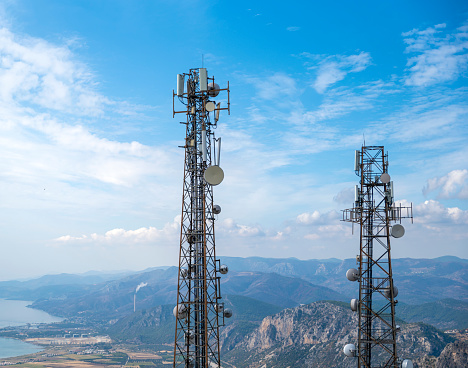
\includegraphics[width=\textwidth]{figures/power_lines.jpg}
        \end{column}
        
    \end{columns}
\end{frame}

\begin{frame}{Como modelar isso com grafos?}
    \begin{itemize}
        \item Cada torre de celular é representada por um \textbf{vértice}.
        
        \item Se duas torres estão próximas (na mesma região de cobertura), conectamos os vértices com uma \textbf{aresta}, porque elas \textbf{não podem usar a mesma frequência}.
        
        \item Atribuímos uma \textbf{``cor''} para cada vértice, representando uma \textbf{frequência de transmissão}. O objetivo é \textbf{minimizar} o número de frequências diferentes, mas garantindo que torres próximas \textbf{não tenham a mesma cor}.
    \end{itemize}
\end{frame}
\section{Representações de Grafos}

\begin{frame}{Lista de Adjacência}
    Um grafo $G=(V,E)$ é representado por um arranjo de listas. Para cada vértice $u \in V$, há uma lista que contém todos os seus vizinhos.
    
    $$ \text{Adj}(u) = \{ v \in V \mid (u, v) \in E \} $$
    
    \pause % <-- O slide para aqui até você avançar
    
    \textbf{Pontos Fortes}
    \begin{itemize}
        \item<+-> Eficiência de Espaço: Ideal para grafos com poucas arestas (esparsos). O espaço usado é proporcional ao número de vértices e arestas: $O(|V|+|E|)$.
        \item<+-> Busca de Vizinhos Rápida: Listar todos os vizinhos de um vértice é muito eficiente.
    \end{itemize}

    \pause % <-- O slide para aqui até você avançar
    
    \textbf{Pontos Fracos}
    \begin{itemize}
        \item<+-> Verificação de Aresta Lenta: Checar se a aresta (u,v) existe pode exigir a varredura de toda a lista de vizinhos de u.
    \end{itemize}
\end{frame}

\begin{frame}{Matriz de Adjacência}
    Um grafo com $n$ vértices é representado por uma matriz quadrada $M$ de dimensão $n \times n$.
    
    $$
    M_{uv} =
    \begin{cases}
        1 & \text{se existe a aresta } (u, v), \\
        0 & \text{caso contrário.}
    \end{cases}
    $$
    
    \pause % Primeira pausa
    
    \textbf{Pontos Fortes}
    \begin{itemize}
        \item<+-> Verificação de Aresta Instantânea: Saber se a aresta (u,v) existe é uma operação de tempo constante: $O(1)$.
        \item<+-> Adição/Remoção Rápida de Arestas: Alterar o valor na matriz de 0 para 1 (ou vice-versa) é muito rápido.
    \end{itemize}    

    \pause % <-- O slide para aqui até você avançar
    
    \textbf{Pontos Fracos}
    \begin{itemize}
        \item<+-> Alto Custo de Memória: O espaço é sempre $O(|V|^2)$, mesmo para grafos com poucas arestas, o que gera desperdício.
    \end{itemize}
\end{frame}

\begin{frame}{Exemplo: Sugestão de Amigos em Rede Social}
    \textbf{O Problema:} Para um usuário, encontrar seus "amigos de amigos" para sugerir novas conexões.
    
    \pause % Pausa 1
    
    \begin{itemize}
        \item \textbf{Modelo:} Um grafo com 1 milhão de vértices (usuários).
        \item \textbf{Característica:} Grafo \textit{esparso}, onde cada usuário tem em média 200 amigos (arestas).
    \end{itemize}
    
    \pause % Pausa 2
    
    \textbf{Abordagem 1: Usando Lista de Adjacências}
    \begin{itemize}
        \item<+-> \textbf{Passo 1:} Acessar a lista do usuário inicial. Custo: ler 200 nomes.
        \item<+-> \textbf{Passo 2:} Para cada um desses 200 amigos, acessar suas respectivas listas (com ~200 nomes cada).
    \end{itemize}
    
    \pause % Pausa 3
    
    \begin{block}{Custo Computacional}
        O número de operações é proporcional às conexões reais:
        $$ \approx 200 \times 200 = \textbf{40.000 operações (rápido e eficiente)} $$
    \end{block}

\end{frame}

\begin{frame}{Análise Comparativa e Conclusão}
    
    \textbf{Abordagem 2: Usando Matriz de Adjacências}
    
    \begin{itemize}
        \item<+-> \textbf{Custo de Memória:} Exigiria uma matriz de $10^6 \times 10^6$, ou seja, $10^{12}$ células. \textbf{Totalmente inviável!}
        \item<+-> \textbf{Custo de Computação:} Para achar os amigos de alguém, é preciso varrer 1 milhão de colunas.
            $$ \approx 200 \times 1.000.000 = \textbf{200 milhões de operações} $$
    \end{itemize}

    \pause % Pausa 1
    
    \begin{block}{Tabela Comparativa}
    \centering
    \begin{tabular}{r c c}
        \hline
        \textbf{Critério} & \textbf{Lista de Adjacências} & \textbf{Matriz de Adjacências} \\
        \hline
        Memória & Mínima ($O(|V|+|E|)$) & Gigantesca ($O(|V|^2)$) \\
        Velocidade & Quase Instantâneo & Extremamente Lento \\
        \hline
    \end{tabular}
    \end{block}
    
    \pause % Pausa 2

    \textbf{Conclusão:} Para grafos esparsos do mundo real, a \textbf{Lista de Adjacências} é a única escolha computacionalmente viável e eficiente.

\end{frame}

\begin{frame}{Exemplo de IA: Análise de Relações em Textos}
    \textbf{O Problema:} Um modelo de IA (como os que equipam a busca do Google ou o ChatGPT) precisa aprender a relação semântica entre as palavras mais importantes de um idioma.

    \pause % Pausa 1
    
    \begin{itemize}
        \item \textbf{Modelo:} Um grafo com os \textbf{5.000 termos} mais comuns de um vocabulário.
        \item \textbf{Característica:} Grafo \textit{denso}. Palavras como "governo" ou "economia" se conectam com milhares de outras.
        \item \textbf{Operação Crítica:} Durante o treinamento, o modelo precisa verificar milhões de vezes e de forma \textbf{instantânea} se dois termos, como ('ciência', 'dados'), possuem uma conexão direta.
    \end{itemize}
    
    \pause % Pausa 2
    
    \textbf{Abordagem 1: Usando Matriz de Adjacências}
    \begin{itemize}
        \item<+-> \textbf{Estrutura:} Uma matriz $5000 \times 5000$. O espaço de memória é alto, mas fixo e perfeitamente gerenciável para este porte.
        \item<+-> \textbf{Verificação de Aresta:} Para checar a conexão ('ciência', 'dados'), o acesso é direto à célula \texttt{M[id\_ciencia][id\_dados]}.
    \end{itemize}
\end{frame}        

\begin{frame}{Exemplo de IA: Análise de Relações em Textos}
    \begin{block}{Custo Computacional}
        A verificação da existência de uma aresta é em tempo constante:
        $$ O(1) $$        
    \end{block}
\end{frame}

\begin{frame}{Análise Comparativa e Conclusão (Grafos Densos)}
    \textbf{Abordagem 2: Usando Lista de Adjacências (Neste Cenário)}
    \begin{itemize}
        \item \textbf{Verificação de Aresta:} Para checar a conexão ('ciência', 'dados'), o algoritmo precisaria:
        \begin{enumerate}
            \item Ir para a lista de vizinhos da palavra 'ciência'.
            \item Percorrer \textbf{toda a lista} (que pode ter milhares de palavras) para procurar por 'dados'.
        \end{enumerate}
        \item<+-> \textbf{Custo:} $O(\text{grau}(\text{ciência}))$. Em um grafo denso, isso significa \textbf{milhares de operações para uma única verificação}, o que tornaria o treinamento da IA extremamente lento.
    \end{itemize}
    
    \pause % Pausa 1
    
    \begin{block}{Tabela Comparativa (Para este Cenário de IA)}
        \centering
        \begin{tabular}{r c c}
            \hline
            \textbf{Critério} & \textbf{Matriz de Adjacências} & \textbf{Lista de Adjacências} \\
            \hline
            Verif. de Aresta & \textbf{Instantâneo ($O(1)$)} & Lento ($O(grau)$) \\
            Uso em IA & \textbf{Ideal para treino} & Ineficiente para treino \\
            \hline
        \end{tabular}
    \end{block}
    
    \pause % Pausa 2
    
    \textbf{Conclusão:} Para grafos \textbf{densos} e checagens de arestas em \textbf{$O(1)$}, a \textbf{Matriz de Adjacências} é a mais eficiente.
\end{frame}
\section{Força Bruta x Heurística de Grundy}
\section{Resultados de Desempenho}

\begin{frame}{Estratégia de Execução Paralela com OpenMP}
    Para otimizar o tempo total da coleta de dados, utilizamos a biblioteca \texttt{OpenMP} do C++ para executar os benchmarks em paralelo.

    \vspace{0.5cm}

    \begin{itemize}
        \item A carga de trabalho foi dividida em 3 tarefas independentes, uma para cada tamanho de grafo a ser testado.

        \item As três tarefas, correspondentes a:
            \begin{itemize}
                \item \textbf{n = 500}
                \item \textbf{n = 1000}
                \item \textbf{n = 2000}
            \end{itemize}
        
        \item foram executadas simultaneamente na mesma máquina, aproveitando os múltiplos núcleos do processador para reduzir o tempo total de espera.
    \end{itemize}
\end{frame}

\begin{frame}{Ambiente de Teste}
    \frametitle{Hardware Utilizado}
    \begin{columns}[T]
        % Coluna da Esquerda com a imagem
        \begin{column}{0.55\textwidth}
            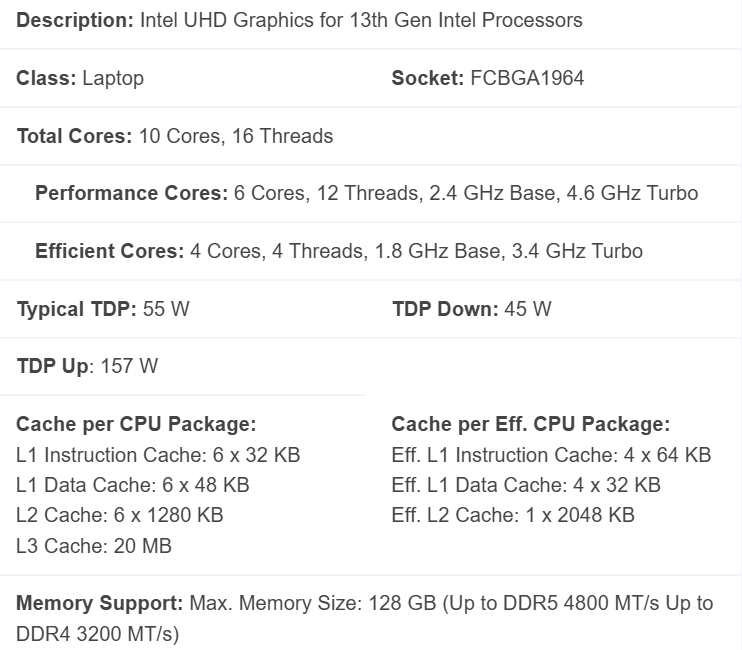
\includegraphics[width=\textwidth]{figures/processor.png}
        \end{column}
        
        % Coluna da Direita com as especificações detalhadas
        \begin{column}{0.6\textwidth}
            \textbf{Processador i5 13450HX (Laptop)}
            \vspace{0.2cm}
            \begin{itemize}
                \item \textbf{Arquitetura Híbrida:}
                    \begin{itemize}
                        \item 6 Núcleos de Performance (até 4.6 GHz) com 12 Threads
                        \item 4 Núcleos de Eficiência (até 3.4 GHz) com 4 Threads
                        \item \textbf{Total:} 10 Núcleos e 16 Threads
                    \end{itemize}
                \item \textbf{Memória Cache:}
                    \begin{itemize}
                        \item L3 Total: 20 MB
                        \item L2 Total: 9.5 MB
                    \end{itemize}
                \item \textbf{Memória Suportada:}
                    \begin{itemize}
                        \item DDR5 até 4800 MT/s
                        \item DDR4 até 3200 MT/s
                    \end{itemize}
            \end{itemize}
        \end{column}
    \end{columns}
\end{frame}


\begin{frame}{Desempenho do Algoritmo de Força Bruta (nanossegundos)}
    \centering
    { % Inicia um grupo para a mudança ser local
    \renewcommand{\arraystretch}{1.5} % <-- AQUI ESTÁ A MÁGICA!
    \begin{tabular}{|c|r|r|}
        \hline
        \textbf{N (Vértices)} & \textbf{Lista (ns)} & \textbf{Matriz (ns)} \\
        \hline
        8 & 68,833.60 & 2,428.82 \\
        \hline
        10 & 200,551.00 & 3,104.70 \\
        \hline
        12 & 655,799.00 & 3,146.28 \\
        \hline
        14 & 2,090,960.00 & 3,384.53 \\
        \hline
    \end{tabular}
    } % Termina o grupo
\end{frame}

\begin{frame}{Desempenho da Heurística de Grundy (milissegundos)}
    \centering
    { % Inicia um grupo para a mudança ser local
    \renewcommand{\arraystretch}{1.5} % <-- Aumenta a altura da linha
    \begin{tabular}{|c|r|r|}
        \hline
        \textbf{N (Vértices)} & \textbf{Lista (ms)} & \textbf{Matriz (ms)} \\
        \hline
        500 & 5.34 & 47.92 \\
        \hline
        1000 & 21.51 & 192.57 \\
        \hline
        2000 & 90.64 & 566.79 \\
        \hline
    \end{tabular}
    } % Termina o grupo
\end{frame}

\begin{frame}{Desempenho do Algoritmo de Força Bruta por Representação}
    \centering
    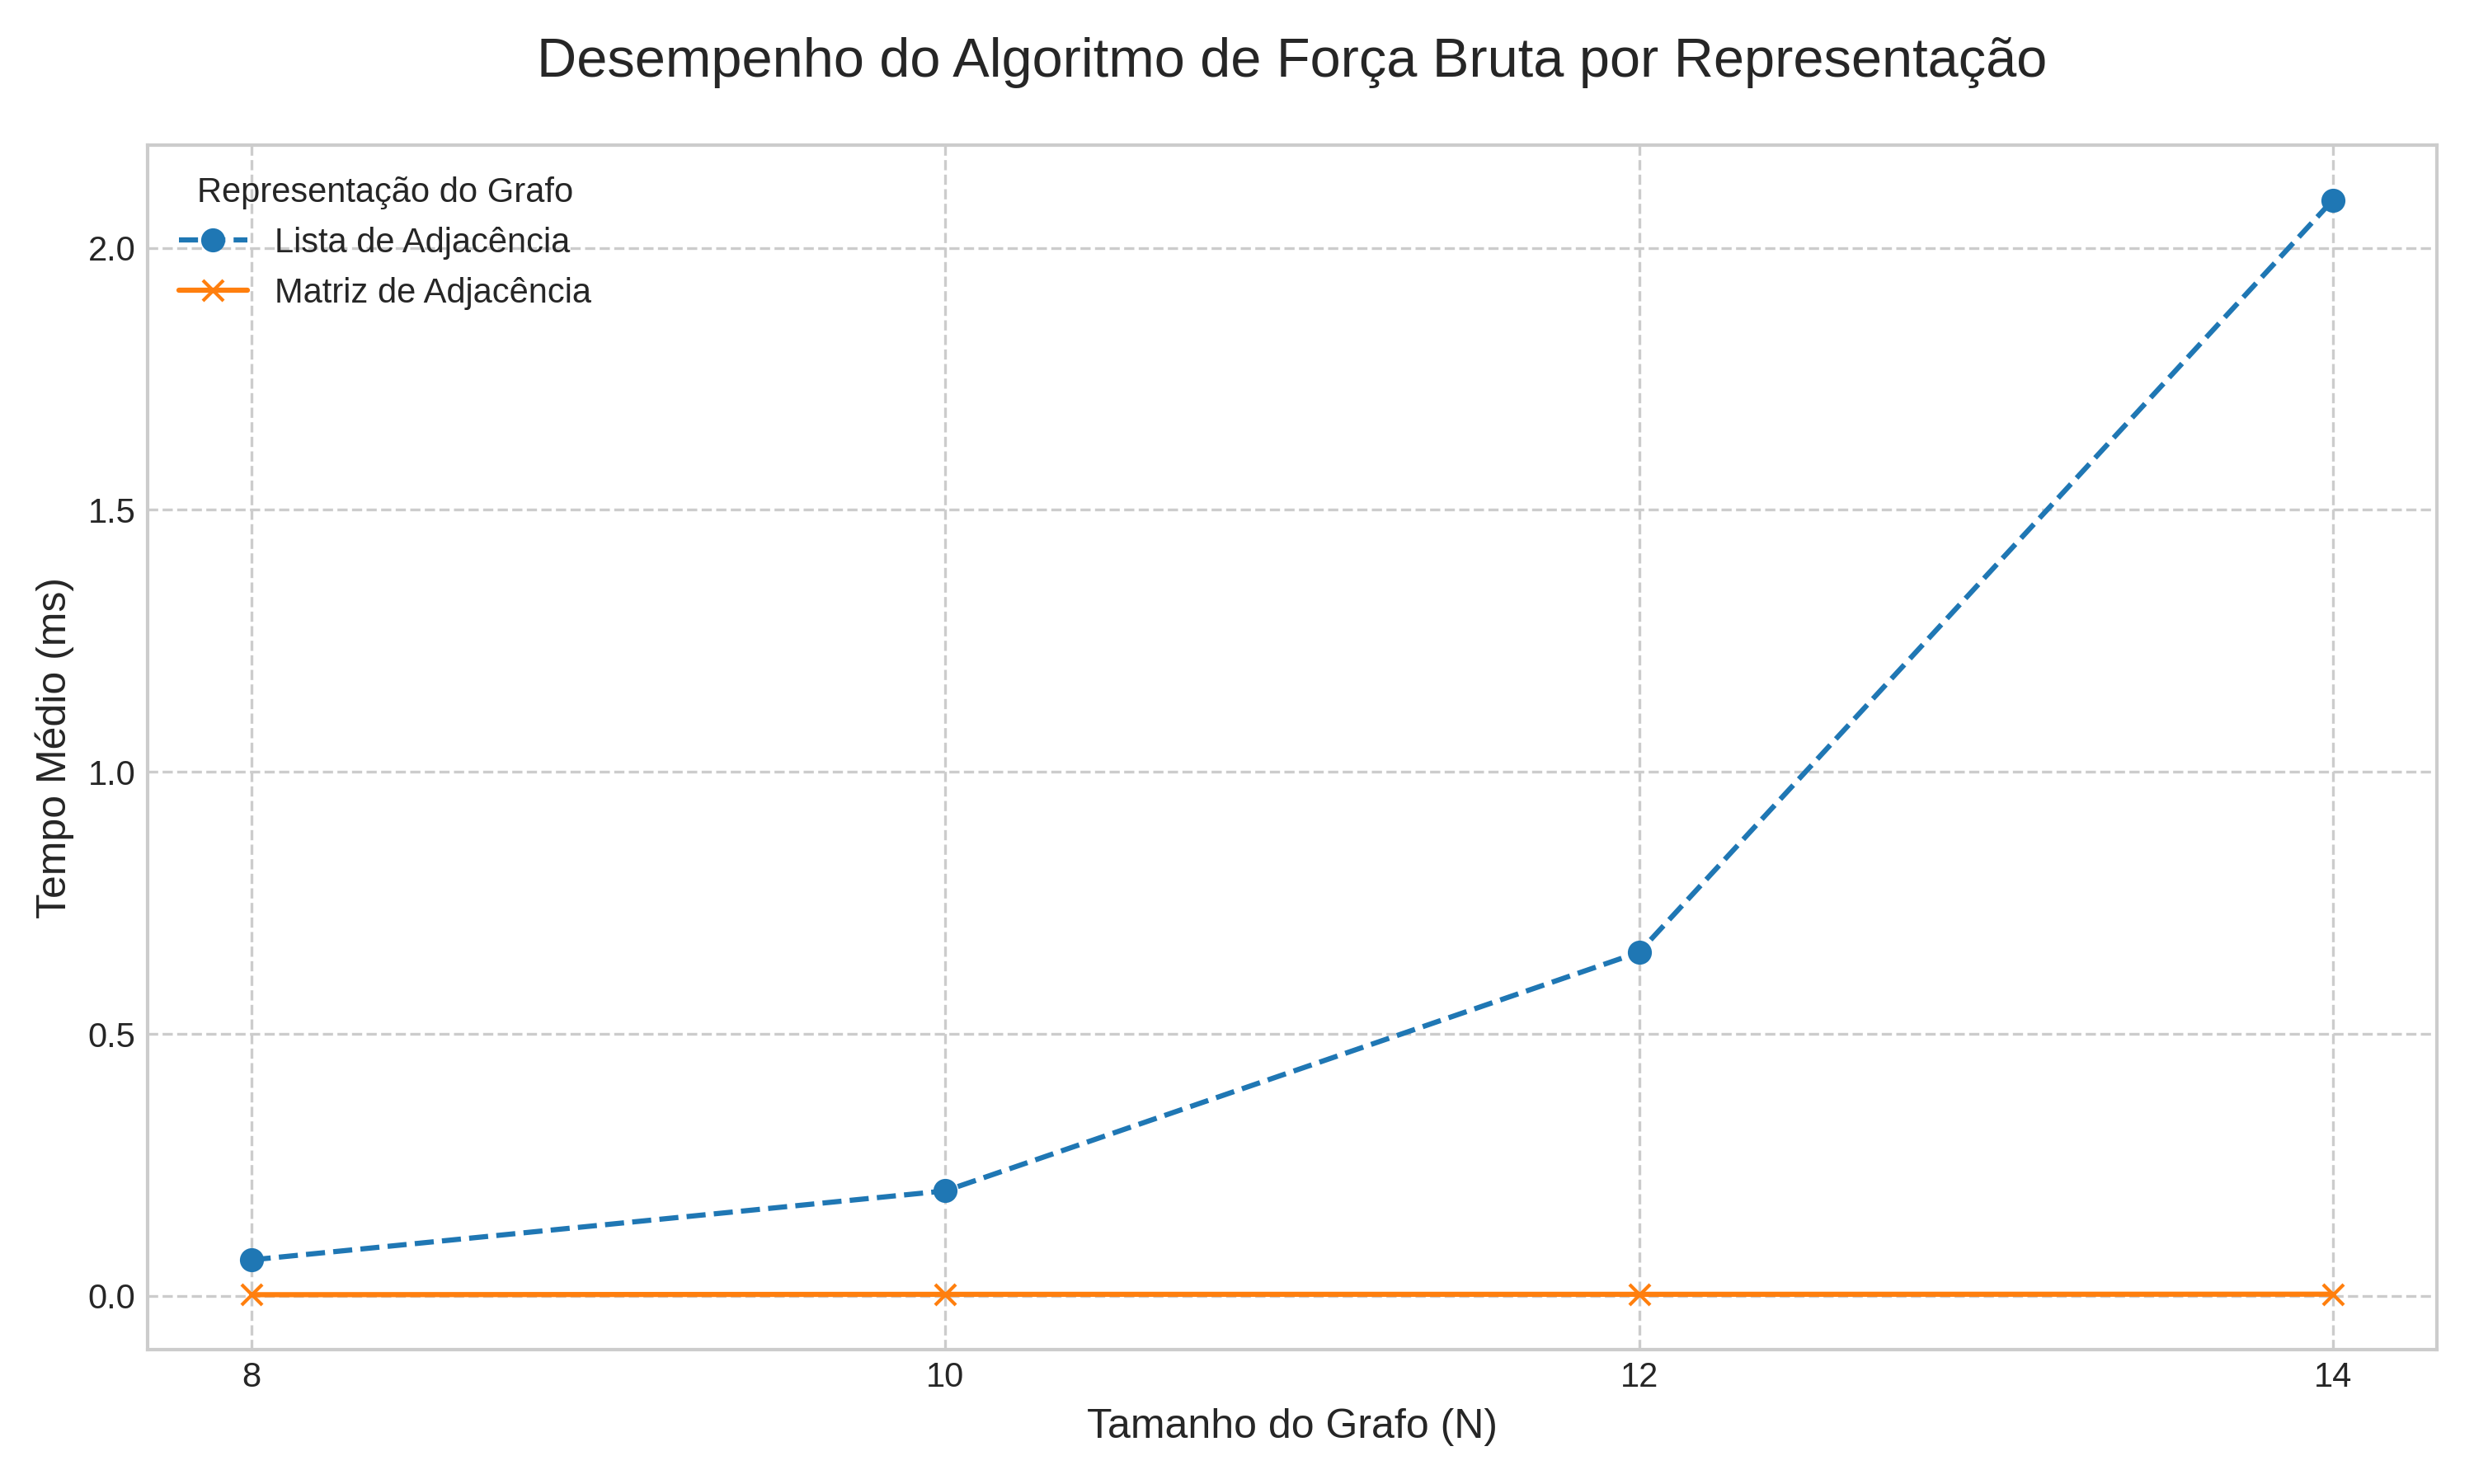
\includegraphics[width=0.9\textwidth]{figures/forca_bruta_comparativo.png}
\end{frame}

\begin{frame}{Desempenho do Algoritmo de Grundy por Representação}
    \centering
    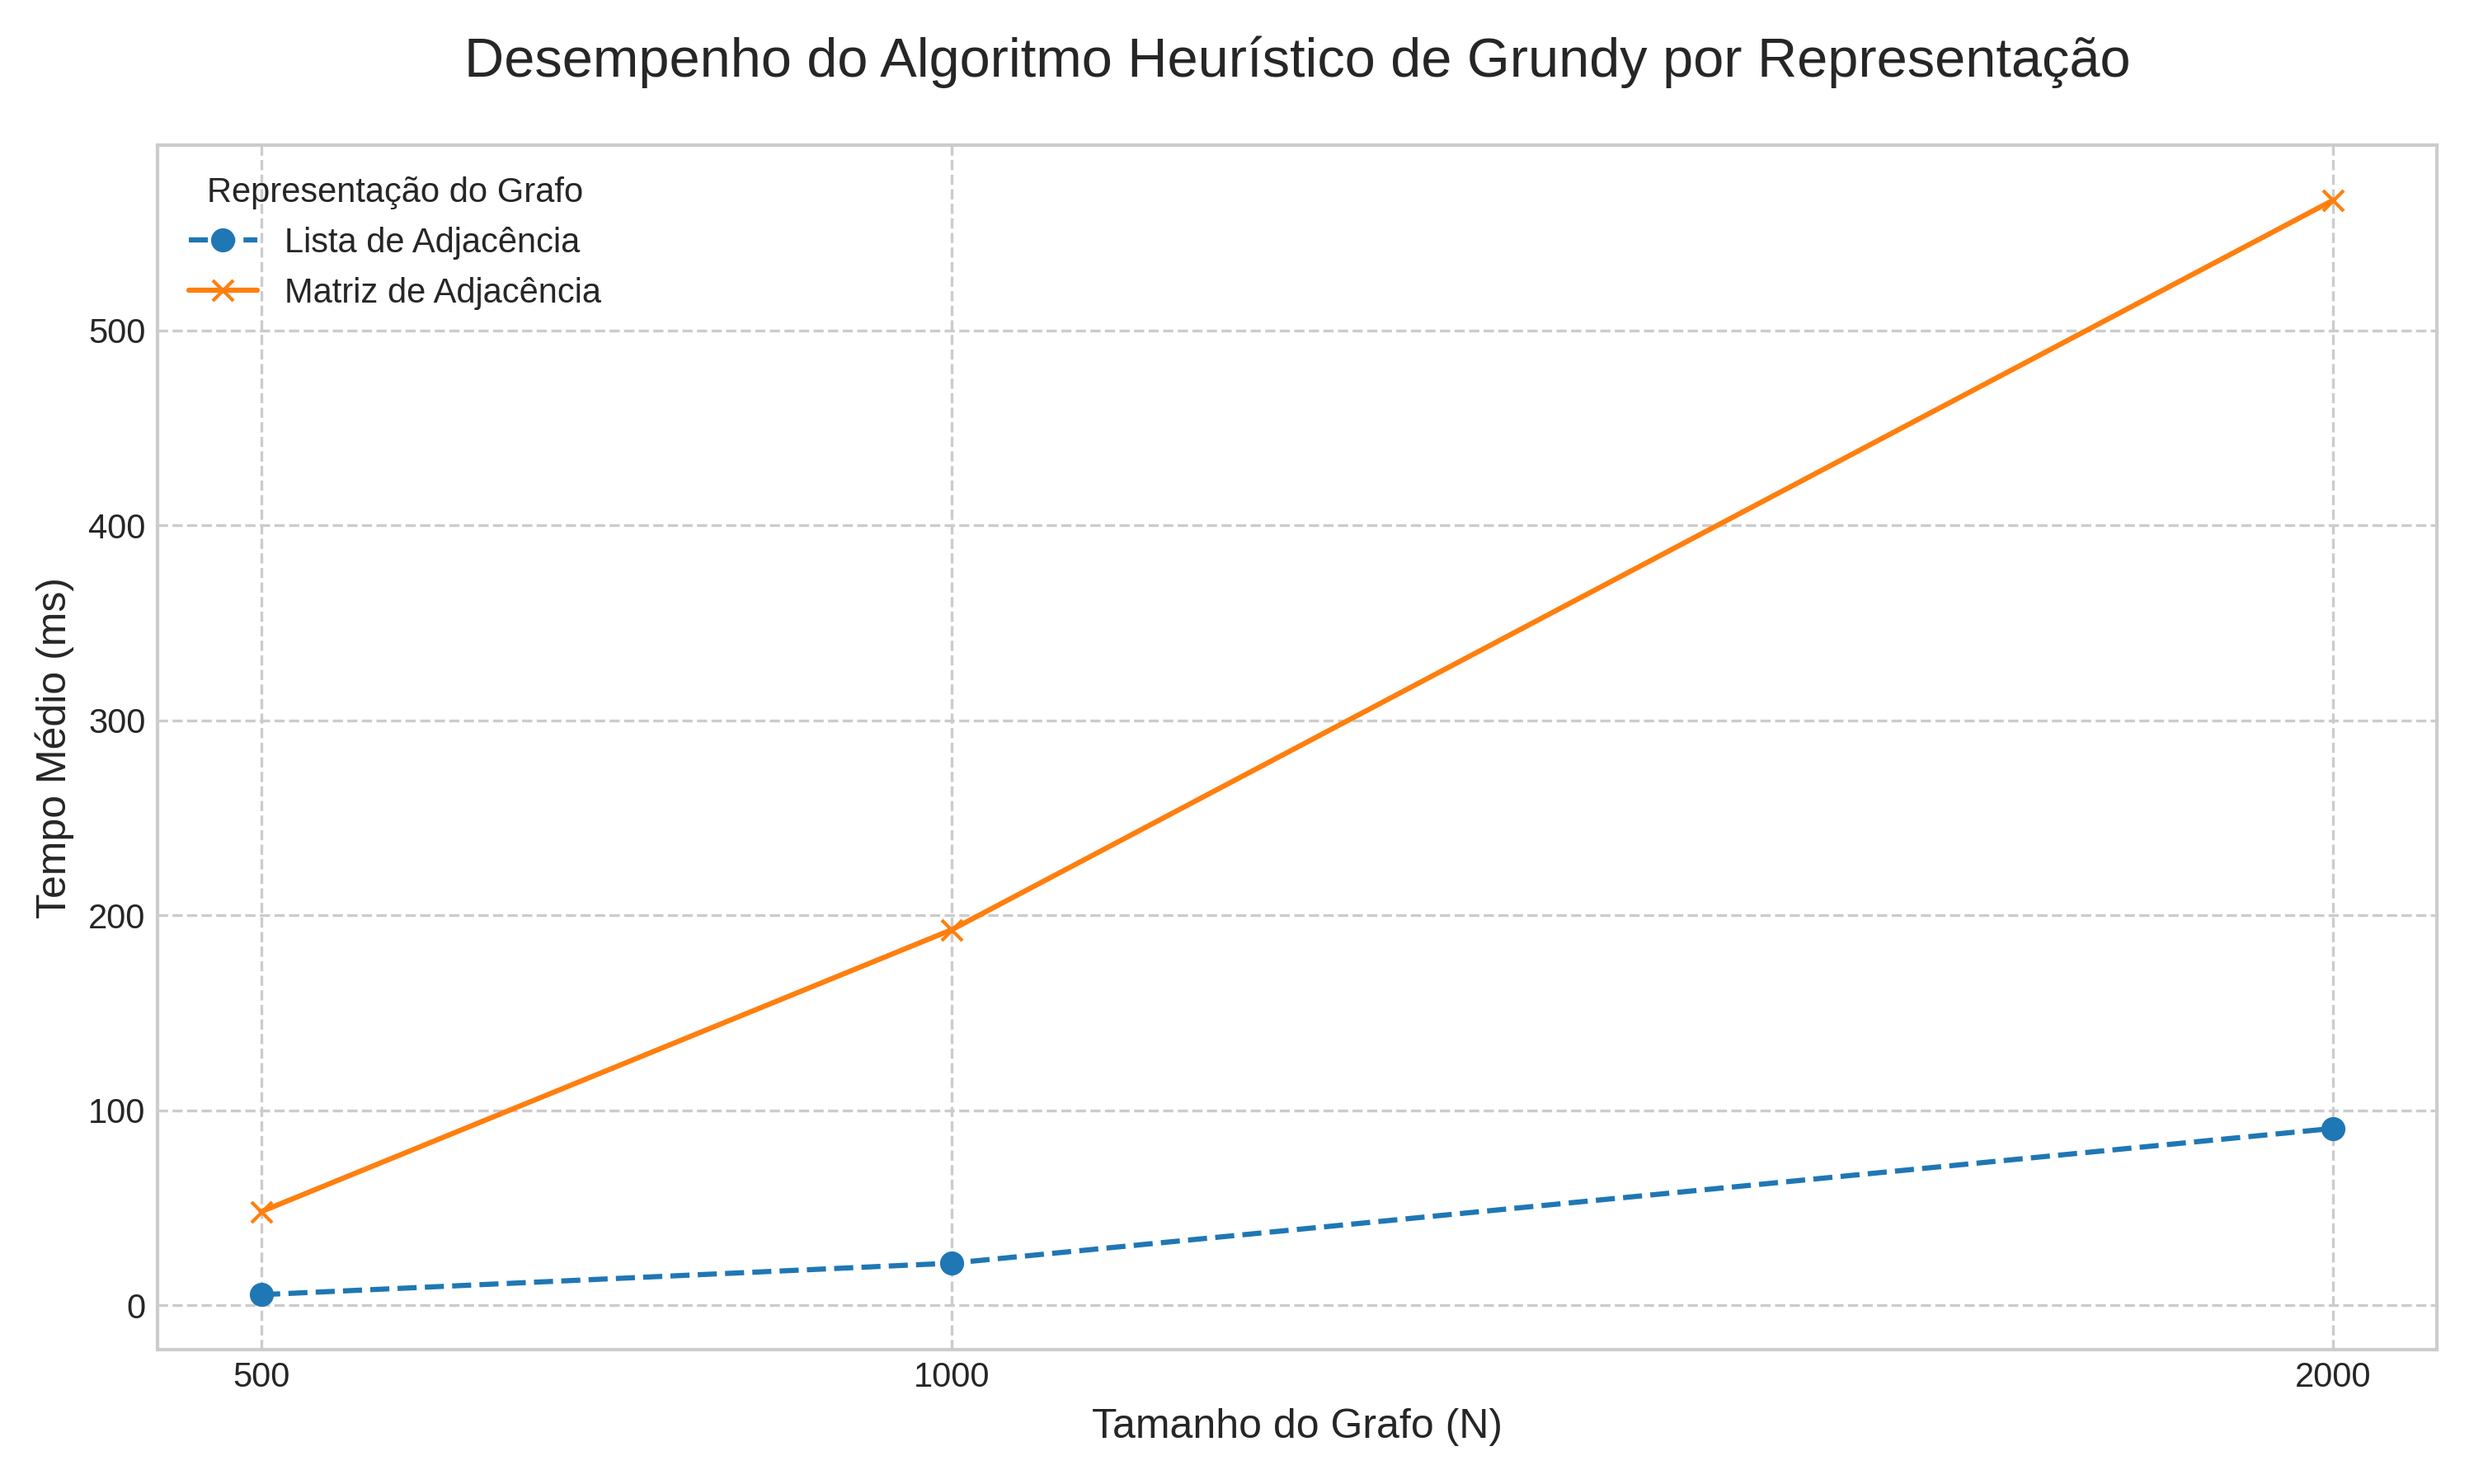
\includegraphics[width=0.9\textwidth]{figures/grundy_comparativo.png}
\end{frame}

\begin{frame}{Estimativas de Tempo para a Fase Grundy}
    \begin{itemize}
        \item Para 1.000 repetições (10 vezes mais que 100):
        \begin{itemize}
            \item $1,1 \text{ minutos} \times 10 = 11 \text{ minutos}$
        \end{itemize}
        
        \vspace{0.4cm}
        
        \item Para 10.000 repetições (100 vezes mais que 100):
        \begin{itemize}
            \item $1,1 \text{ minutos} \times 100 = 110 \text{ minutos}$
            \item Isso é aproximadamente 1 hora e 50 minutos.
        \end{itemize}
        
        \vspace{0.4cm}
        
        \item Para 1.000.000 de repetições (10.000 vezes mais que 100):
        \begin{itemize}
            \item $1,1 \text{ minutos} \times 10.000 = 11.000 \text{ minutos}$
            \item Convertendo para horas: $11.000 / 60 \approx 183,3 \text{ horas}$
            \item Convertendo para dias: $183,3 / 24 \approx 7,6 \text{ dias}$
        \end{itemize}
    \end{itemize}
\end{frame}
\section{Conclusão}

\begin{frame}{Conclusões \& programação competitiva}
    \begin{enumerate}
        \item Inviabilidade da força bruta
        \item Heurísticas como solução adequada
        \item Lista de Adjacência como escolha preferencial
        \item Análise de restrições
    \end{enumerate}
\end{frame}
\section{Referências Bibliográficas}

\begin{frame}[allowframebreaks]
    \frametitle{Referências Bibliográficas}

    \begin{thebibliography}{99}

        \bibitem{cormen}
        CORMAN, T. H.; LEISERSON, C. E.; RIVEST, R. L.; STEIN, C. \textit{Algoritmos: Teoria e Prática}. 3ª ed. Campus, 2012.        

        \bibitem{sedgewick}
        SEDGEWICK, R.; WAYNE, K. \textit{Algorithms}. 4ª ed. Addison-Wesley Professional, 2011.        

        \bibitem{diestel}
        DIESTEL, R. \textit{Graph Theory}. 5ª ed. Springer, 2017.        

        \bibitem{bondy}
        BONDY, J. A.; MURTY, U. S. R. \textit{Graph Theory}. Springer, 2008.        

        \bibitem{skiena}
        SKIENA, S. S. \textit{The Algorithm Design Manual}. 2ª ed. Springer, 2008.        

    \end{thebibliography}

\end{frame}

\end{document}

% Slide final
\begin{frame}
\begin{center}
{\Huge Obrigado pela atenção!}
\vspace{1cm}

\end{center}
\end{frame}

\end{document}
